% Success! Your submission appears on this page. The submission confirmation number is 82131458-2aa0-47a3-9f75-662ac51d9301. Copy and save this number as proof of your submission.

\documentclass{article}
\usepackage[utf8]{inputenc}
\usepackage{multicol}
\usepackage{listings}
\usepackage{amssymb}
\usepackage{enumitem}
\usepackage{graphicx}
\usepackage{amsthm}
\usepackage{hyperref}
\usepackage{tikz}
\usepackage{amsmath}
\usepackage[ruled, vlined]{algorithm2e}
\usepackage{mathtools}
\newtheorem{theorem}{Theorem}
\newtheorem{definition}{Definition}
\newcommand{\N}{\mathbb{N}}
\newcommand{\Np}{{\mathbb{N}^{>0}}}
\newcommand{\Z}{\mathbb{Z}}
\newcommand{\R}{\mathbb{R}}
\newcommand{\bigO}{\mathcal{O}}
\newcommand{\code}[1]{\texttt{#1}}
\newcommand{\hints}[1]{\paragraph{\bf Hints:} #1}

\SetKwProg{Fn}{Function}{}{}
\SetKwProg{Proc}{Procedure}{}{}
\SetKwFunction{FloydWarshall}{FloydWarshall}
\SetKwFunction{print}{print}
\SetKwFunction{newline}{newline}
\SetKwFunction{maxProfitCalculator}{maxProfitCalculator}

\usetikzlibrary{arrows, positioning}

\begin{document}

\title{Algorithms \& Datastructures \\ Weekly Assignment 12}
\date{\today}
\author{Tony Lopar \\ s1013792}
\maketitle
\section*{Exercise 1}
% Because the MST takes the tree of edges of which the sum costs the minimum, the minimum weight edges are added first to the tree. The MST will always contain a minimum weight edge, because if we would take only edges of a higher weight than the mimimum weight, there is a combination of smaller edges possible, so the tree won't be an actual MST in that case.

Let's assume that the following graph is a subgraph of a possible bigger graph and that the edge ab with weight 3 is the edge with mimimum weight.
 % MST contains no edge of minimum weight. If an edge is the only edge to a vertex, it should be added to the tree, since otherwise the graph is not connected anymore. In the case that the edge of minimum weight may form a cycle we may have a subgraph as follows in the graph:

\begin{center}
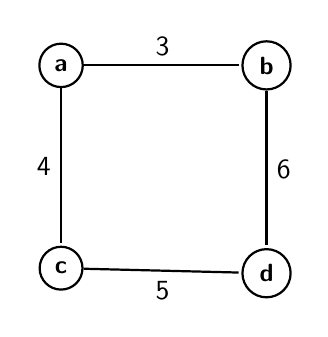
\begin{tikzpicture}[-,>=stealth',shorten >=1pt,auto,node distance=2cm, every loop/.style={},
                    thick, ,main node/.style={circle,draw,font=\sffamily\small\bfseries}]

  \node[main node] (1) {a};
  \node[main node] (2) [right=2cm and 2cm of 1] {b};
  \node[main node] (3) [below=2cm and 4cm of 1] {c};
  \node[main node] (4) [below=2cm and 4cm of 2] {d};

  \path[every node/.style={font=\sffamily\normalsize, text = black }]
    (1) edge[black] node [above] {3} (2)
        edge[black] node [left] {4} (3)
    (2) edge[black] node [right] {6} (4)
    (3) edge[black] node [below] {5} (4);
\end{tikzpicture}
\end{center}
If the MST doesn't contains the edge ab, then there will be a spanning tree possible with a lower sum of cost which means it isn't the actual MST then. In the graph above in this case the edges ac, bd and cd will be in the tree. However, we see that if we replace the edge bd with ab we have a tree with a cost that's tree lower. The tree will still remain intact since we still may reach d from b. This example may be generalized to all cyclic subgraph which means that if there is no edge of minimum weight in the MST, then the cost of the MST isn't the actual minimum.


\section*{Exercise 2}
\begin{enumerate}
  \item For each iteration the vertex added to the spanning tree will be colored in the graph.
  I chose node a as the initialization node. In the first iteration we add the edge with the smallest weight that's having an endpoint in a to the tree. In this case it's the edge ad with weight 3. We colour this blue and add a and d to S. After this iteration the priority queue will contain the vertices b, e and c. The only vertex with a predecessor currently is D which has A as predecessor and itself as key.
  \begin{center}
  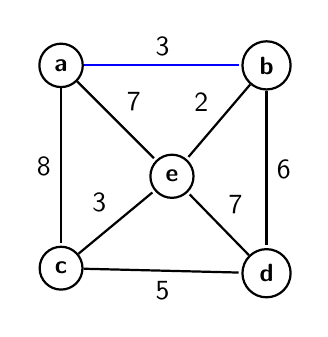
\begin{tikzpicture}[-,>=stealth',shorten >=1pt,auto,node distance=2cm, every loop/.style={},
                      thick, ,main node/.style={circle,draw,font=\sffamily\small\bfseries}]

    \node[main node] (1) {a};
    \node[main node] (2) [right=2cm and 2cm of 1] {b};
    \node[main node] (3) [below=2cm and 4cm of 1] {c};
    \node[main node] (4) [below=2cm and 4cm of 2] {d};
    \node[main node] (5) [below right=1cm and 1cm of 1] {e};

    \path[every node/.style={font=\sffamily\normalsize, text = black }]
      (1) edge[blue] node [above] {3} (2)
          edge[black] node [left] {8} (3)
          edge[black] node [above right] {7} (5)
      (2) edge[black] node [right] {6} (4)
          edge[black] node [above left] {2} (5)
      (3) edge[black] node [below] {5} (4)
          edge[black] node [above left] {3} (5)
      (4) edge[black] node [above right] {7} (5);
  \end{tikzpicture}
  \end{center}
  In the next iteration we will add the egde be to the tree, since this is the edge with the smallest weight with an endpoint in the current tree. After this iteration the priority queue will contain the vertices e, d and c. The vertex A will get the b as predecessor assigned.
  \begin{center}
  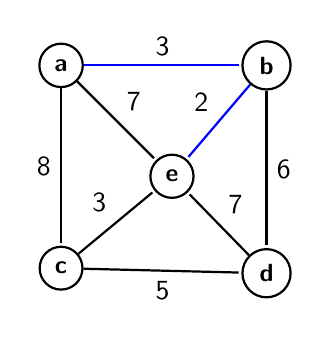
\begin{tikzpicture}[-,>=stealth',shorten >=1pt,auto,node distance=2cm, every loop/.style={},
                      thick, ,main node/.style={circle,draw,font=\sffamily\small\bfseries}]

    \node[main node] (1) {a};
    \node[main node] (2) [right=2cm and 2cm of 1] {b};
    \node[main node] (3) [below=2cm and 4cm of 1] {c};
    \node[main node] (4) [below=2cm and 4cm of 2] {d};
    \node[main node] (5) [below right=1cm and 1cm of 1] {e};

    \path[every node/.style={font=\sffamily\normalsize, text = black }]
      (1) edge[blue] node [above] {3} (2)
          edge[black] node [left] {8} (3)
          edge[black] node [above right] {7} (5)
      (2) edge[black] node [right] {6} (4)
          edge[blue] node [above left] {2} (5)
      (3) edge[black] node [below] {5} (4)
          edge[black] node [above left] {3} (5)
      (4) edge[black] node [above right] {7} (5);
  \end{tikzpicture}
  \end{center}

In the next iteration we will add the egde ce to the tree, since this is the edge with the smallest weight with an endpoint in the current tree. After this iteration the priority queue will contain the vertices c and d. Vertex C will have E assigned as predecessor.
\begin{center}
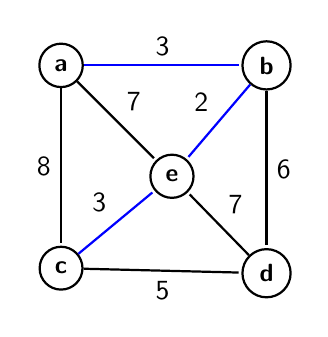
\begin{tikzpicture}[-,>=stealth',shorten >=1pt,auto,node distance=2cm, every loop/.style={},
                    thick, ,main node/.style={circle,draw,font=\sffamily\small\bfseries}]

  \node[main node] (1) {a};
  \node[main node] (2) [right=2cm and 2cm of 1] {b};
  \node[main node] (3) [below=2cm and 4cm of 1] {c};
  \node[main node] (4) [below=2cm and 4cm of 2] {d};
  \node[main node] (5) [below right=1cm and 1cm of 1] {e};

  \path[every node/.style={font=\sffamily\normalsize, text = black }]
    (1) edge[blue] node [above] {3} (2)
        edge[black] node [left] {8} (3)
        edge[black] node [above right] {7} (5)
    (2) edge[black] node [right] {6} (4)
        edge[blue] node [above left] {2} (5)
    (3) edge[black] node [below] {5} (4)
        edge[blue] node [above left] {3} (5)
    (4) edge[black] node [above right] {7} (5);
\end{tikzpicture}
\end{center}

In the next iteration we will add the egde cd to the tree, since this is the edge with the smallest weight with an endpoint in the current tree. After this iteration the priority queue will contain the vertex d. Vertex D will have C assigned as predecessor.
\begin{center}
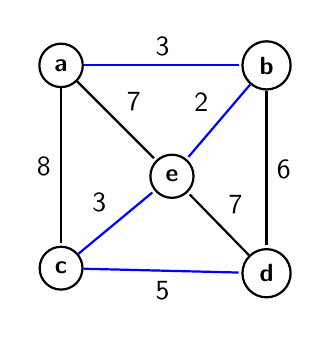
\begin{tikzpicture}[-,>=stealth',shorten >=1pt,auto,node distance=2cm, every loop/.style={},
                    thick, ,main node/.style={circle,draw,font=\sffamily\small\bfseries}]

  \node[main node] (1) {a};
  \node[main node] (2) [right=2cm and 2cm of 1] {b};
  \node[main node] (3) [below=2cm and 4cm of 1] {c};
  \node[main node] (4) [below=2cm and 4cm of 2] {d};
  \node[main node] (5) [below right=1cm and 1cm of 1] {e};

  \path[every node/.style={font=\sffamily\normalsize, text = black }]
    (1) edge[blue] node [above] {3} (2)
        edge[black] node [left] {8} (3)
        edge[black] node [above right] {7} (5)
    (2) edge[black] node [right] {6} (4)
        edge[blue] node [above left] {2} (5)
    (3) edge[blue] node [below] {5} (4)
        edge[blue] node [above left] {3} (5)
    (4) edge[black] node [above right] {7} (5);
\end{tikzpicture}
\end{center}
Now we've reached n-1 edges in the tree, the MST has been completed.
\item In Kruskal's algorithm we will add the edge with the lowest weight in the tree first. This is in this case the edge be. The vertices b and e are added in the MST.
\begin{center}
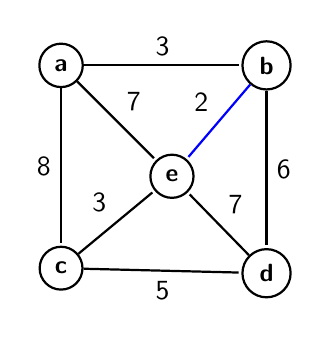
\begin{tikzpicture}[-,>=stealth',shorten >=1pt,auto,node distance=2cm, every loop/.style={},
                    thick, ,main node/.style={circle,draw,font=\sffamily\small\bfseries}]

  \node[main node] (1) {a};
  \node[main node] (2) [right=2cm and 2cm of 1] {b};
  \node[main node] (3) [below=2cm and 4cm of 1] {c};
  \node[main node] (4) [below=2cm and 4cm of 2] {d};
  \node[main node] (5) [below right=1cm and 1cm of 1] {e};

  \path[every node/.style={font=\sffamily\normalsize, text = black }]
    (1) edge[black] node [above] {3} (2)
        edge[black] node [left] {8} (3)
        edge[black] node [above right] {7} (5)
    (2) edge[black] node [right] {6} (4)
        edge[blue] node [above left] {2} (5)
    (3) edge[black] node [below] {5} (4)
        edge[black] node [above left] {3} (5)
    (4) edge[black] node [above right] {7} (5);
\end{tikzpicture}
\end{center}

Next, we continue with the remaining edge with the lowest weight. Both have the weight 3, so we may choose which one should be added first. Therefore we choose ab. We will also add the vertex a to the mst.
\begin{center}
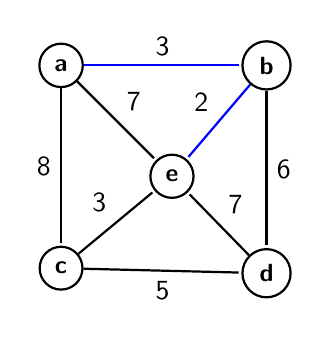
\begin{tikzpicture}[-,>=stealth',shorten >=1pt,auto,node distance=2cm, every loop/.style={},
                    thick, ,main node/.style={circle,draw,font=\sffamily\small\bfseries}]

  \node[main node] (1) {a};
  \node[main node] (2) [right=2cm and 2cm of 1] {b};
  \node[main node] (3) [below=2cm and 4cm of 1] {c};
  \node[main node] (4) [below=2cm and 4cm of 2] {d};
  \node[main node] (5) [below right=1cm and 1cm of 1] {e};

  \path[every node/.style={font=\sffamily\normalsize, text = black }]
    (1) edge[blue] node [above] {3} (2)
        edge[black] node [left] {8} (3)
        edge[black] node [above right] {7} (5)
    (2) edge[black] node [right] {6} (4)
        edge[blue] node [above left] {2} (5)
    (3) edge[black] node [below] {5} (4)
        edge[black] node [above left] {3} (5)
    (4) edge[black] node [above right] {7} (5);
\end{tikzpicture}
\end{center}

Since ce is the edge with the lowest weight remaining we will add this edge to the mst. We will also add the vertex c to the MST.
\begin{center}
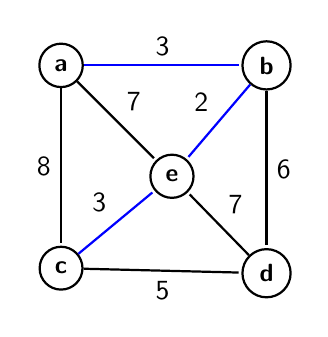
\begin{tikzpicture}[-,>=stealth',shorten >=1pt,auto,node distance=2cm, every loop/.style={},
                    thick, ,main node/.style={circle,draw,font=\sffamily\small\bfseries}]

  \node[main node] (1) {a};
  \node[main node] (2) [right=2cm and 2cm of 1] {b};
  \node[main node] (3) [below=2cm and 4cm of 1] {c};
  \node[main node] (4) [below=2cm and 4cm of 2] {d};
  \node[main node] (5) [below right=1cm and 1cm of 1] {e};

  \path[every node/.style={font=\sffamily\normalsize, text = black }]
    (1) edge[blue] node [above] {3} (2)
        edge[black] node [left] {8} (3)
        edge[black] node [above right] {7} (5)
    (2) edge[black] node [right] {6} (4)
        edge[blue] node [above left] {2} (5)
    (3) edge[black] node [below] {5} (4)
        edge[blue] node [above left] {3} (5)
    (4) edge[black] node [above right] {7} (5);
\end{tikzpicture}
\end{center}

Next, we will add cd to the tree, since this is the edge with the lowest weight. The vertex d is added to the MST.
\begin{center}
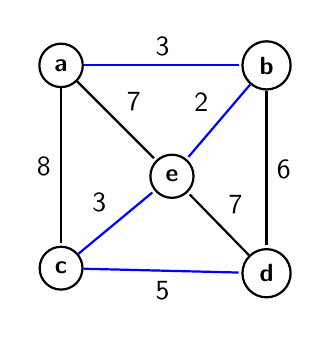
\begin{tikzpicture}[-,>=stealth',shorten >=1pt,auto,node distance=2cm, every loop/.style={},
                    thick, ,main node/.style={circle,draw,font=\sffamily\small\bfseries}]

  \node[main node] (1) {a};
  \node[main node] (2) [right=2cm and 2cm of 1] {b};
  \node[main node] (3) [below=2cm and 4cm of 1] {c};
  \node[main node] (4) [below=2cm and 4cm of 2] {d};
  \node[main node] (5) [below right=1cm and 1cm of 1] {e};

  \path[every node/.style={font=\sffamily\normalsize, text = black }]
    (1) edge[blue] node [above] {3} (2)
        edge[black] node [left] {8} (3)
        edge[black] node [above right] {7} (5)
    (2) edge[black] node [right] {6} (4)
        edge[blue] node [above left] {2} (5)
    (3) edge[blue] node [below] {5} (4)
        edge[blue] node [above left] {3} (5)
    (4) edge[black] node [above right] {7} (5);
\end{tikzpicture}
\end{center}

We see that all other vertices will cause a cycle in the current tree, so we won't add any edge anymore to the tree. This means the tree has been completed.
\item If we turn the array into a binary tree with the middle element of the array as root we may use the algorithm of Prim to sort it. The root will have edges from itselt with the values of the middle two elements of the list as weight. The tree should have the values of the array assigned as the weights of the edges. We will take the root as initial node in Prim's algorithm. The algorithm will first go to the edge with minimum weight with an endpoint in the root. We can place this element as first element in the sorted array. Then the algorithm will take the next smallest value with and endpoint in the tree. This value should be compared with the last value that's already in the list. If it's smaller(so didn't had an endpoint to the tree in a previous iteration) it should be placed on the correct position, otherwise it should be placed at the end of the array. Each iteration will result a sorted array with one element more.

\end{enumerate}

\section*{Exercise 3}
\begin{enumerate}
  \item Yes, the problem is related to the MST since in both cases we would like to find a certain tree that depends on the edge weights in the graph. The great difference is that in a MST we pick the edges with minimum cost and for the MaxST we should pick edges with the heighest cost.
  \item As basis for this algorithm we can take an MST-algorithm like Kruskal for example and modify it to give a MaxST instead of a MST. The modification is that we should add the edges with maximum weight instead of minimum weight to the tree. In the algorithm of Kruskal this would mean that we should sort the edges in a decreasing weight order instead of increasing. The complexity in the case that we take the algorithm of Kruskal will be equal to the algorithm of Kruskal which is $\bigO (m \enspace log \enspace m)$.
\end{enumerate}

\section*{Exercise 4}
Since the supercomputer can only handle one job at a time the total time that the supercomputer is used is equal to the sum of $p_i$ of all jobs. In this time there's no improvement possible. In the time of the computer there is a possible optimization possible. The optimization is that we try to prevent waiting for long jobs on the PC's when all jobs are finished on the supercomputer. Therefore, we should sort the jobs in a decreasing order of $f_i$ and execute them in this order. This will make sure that the waiting time after the jobs on the supercomputer is mimimum since we may execute all jobs parralel on pc's.

After the jobs are sorted, the algorithm may execute in linear time since when the supercomputer finishes a job the next job in the list can be sent to the supercomputer. The total complexity depends on the sorting algorithm that is used to sort the jobs in a decreasing order of $f_i$.

\section*{Exercise 5}
In order to find a possible subsequence in S we should iterate through the m characters of S until we find a character that equals the first character of S' since the subsequence in S should also start with this character. If we found this we will continue to the next character of S and compare it to the next character in S'. If these characters are equal we continue to the next character of both S and S'. If the characters are unequal we only go to the next character of S to compare it. If in the iteration we reached the last character of S' and then we find an equal character, then S' is indeed a subsequence and we should return true. If we iterated through S and haven;t returned true already then S' is no subsequence of S and we return false.

The algorithm is correct since it checks each character of S with the next character of S' that should be equal. If the characters are unequal the character of S is one of the characters that should be removed from S to get the subsequence S'. If in the iteration all characters of S' were equal to a character in S, then we know that the coming characters in S must also be removed to get S'. In the case that the index of S' isn't at the end of the sequence, but we iterated through S then we know that the characters of S' from the pointers are not in the (right order) in S and thus S' is not a subsequence.

\end{document}
